\documentclass[tikz, border=1pt]{standalone}

\usepackage{tikz}
\usetikzlibrary{shapes.arrows, fadings}

\begin{document}
    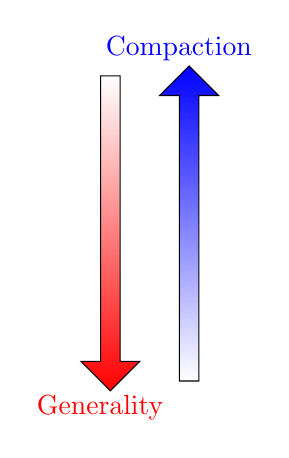
\begin{tikzpicture}
        \node (generality_arrow) at (0, 0) [
            draw=black,
            left color=white,
            single arrow,
            right color=red,
            single arrow,
            minimum height=4cm,
            shading angle=90+270,
            rotate=270
        ] {};
        \path (generality_arrow.south) + (0, -2) node[anchor=north] (generality) {\textcolor{red}{Generality}};
        \path (generality_arrow) + (1, 0) node (compactness_arrow) [
            draw=black,
            left color=white,
            single arrow,
            right color=blue,
            single arrow,
            minimum height=4cm,
            shading angle=90+90,
            rotate=90
        ] {};
        \path (compactness_arrow.north) + (0, 2) node[anchor=south] (generality) {\textcolor{blue}{Compaction}};
    \end{tikzpicture}
\end{document}